\epigraph{If nature is deterministic, a quantum computer could be more than a probability calculator.}{}

\section{Deterministic Quantum Logic}


\begin{figure}[htbp]
\centering
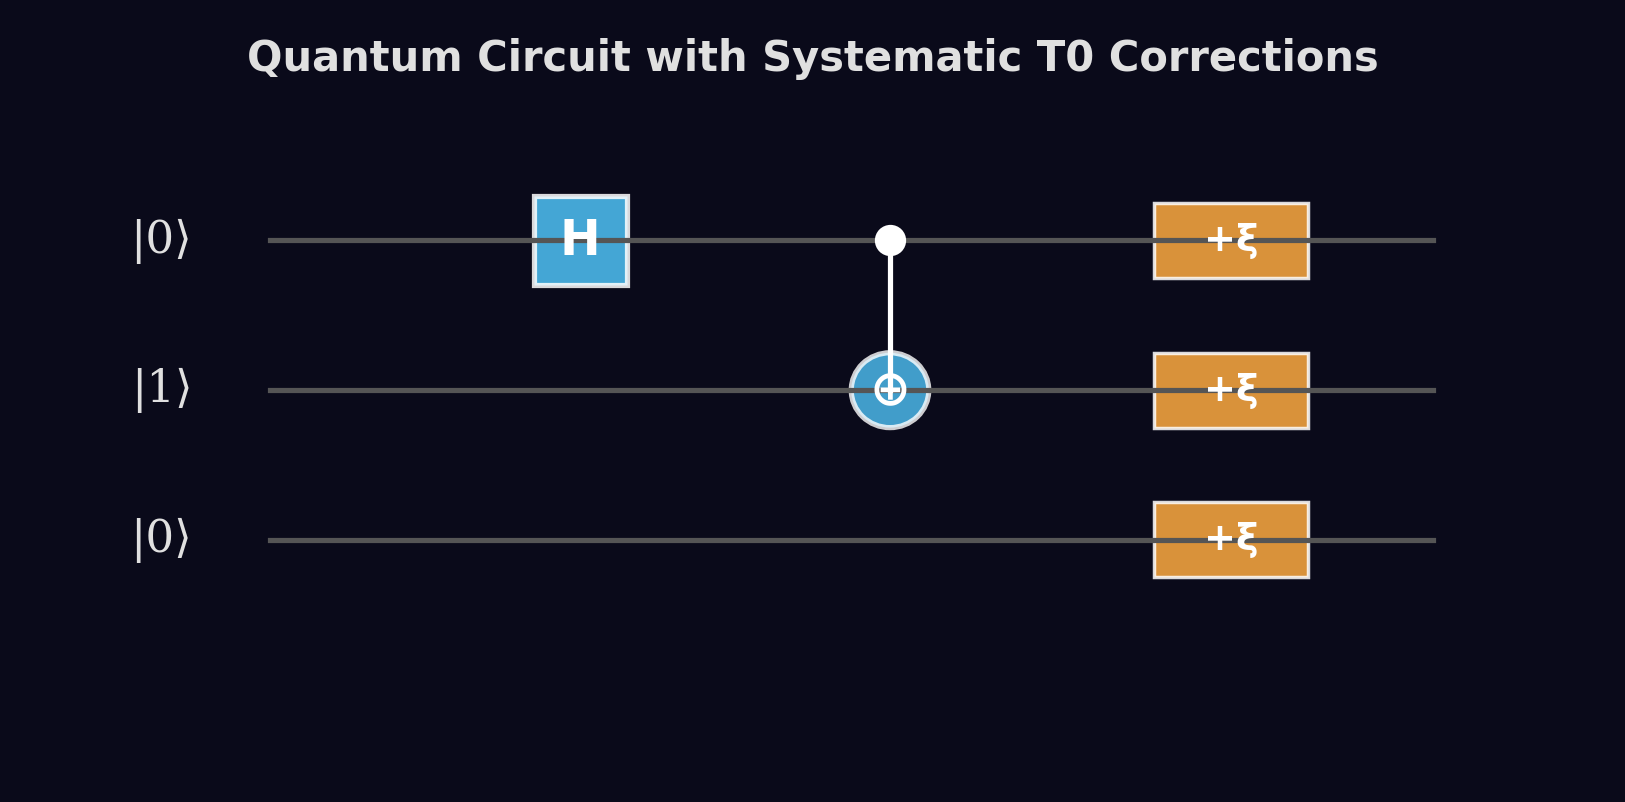
\includegraphics[width=0.85\textwidth]{img/ch10_quantum_circuit.png}
\caption{Quantum circuit with systematic $\xi$ corrections at every gate.}
\end{figure}
The standard interpretation of quantum mechanics says: quantum randomness is fundamental. T0 says something different: \emph{quantum randomness is an illusion of deterministic time-field dynamics.} The consequences for quantum computers are substantial.

\section{T0 Qubits}

In the T0 description, qubits are not probabilistic states but energy-field configurations:
\begin{align}
|0\rangle_{\text{T0}} &\leftrightarrow \delta E_0(x,t) = E_0 \cdot f_0(x,t) \\
|1\rangle_{\text{T0}} &\leftrightarrow \delta E_1(x,t) = E_1 \cdot f_1(x,t)
\end{align}

The basis states are not ``simultaneously present'' in the sense of a genuine superposition. They are different configurations of the vacuum field whose deterministic evolution is so complex that it can \emph{practically} only be described probabilistically.

\section{Modified Quantum Gates}

The T0 corrections to quantum gates are small but measurable. The Hadamard gate receives a $\xsi$ correction:
\begin{equation}
H_{\text{T0}} = H \cdot \left(1 + \xsi \cdot \frac{\langle \delta E \rangle}{E_{\text{Planck}}}\right)
\end{equation}

Shor's algorithm for factorisation improves slightly: $P_{\text{success}}^{\text{T0}} = P_{\text{standard}} \cdot (1 + \xsi\sqrt{n})$. Grover's search algorithm requires fewer iterations: $N_{\text{iter}}^{\text{T0}} = (\pi/4)\sqrt{N} \cdot (1 - \xsi \cdot \ln N)$.

\section{Decoherence Suppression and Bell Corrections}

Particularly promising is the fractal $\xsi$ damping, which provides natural stabilisation against decoherence. And the T0 corrections to Bell inequalities --- CHSH deviations of order~$10^{-3}$ in 73-qubit systems --- are experimentally testable with current technology.

Two fundamental problems of quantum mechanics dissolve in T0: the measurement problem vanishes because there is no wave-function collapse --- only continuous time-field evolution. And the ``spooky action at a distance'' of entanglement becomes local correlation through shared time-field history (cf.\ \href{https://github.com/jpascher/T0-Time-Mass-Duality/blob/main/2/pdf/020_T0_QM-QFT-RT_De.pdf}{Doc.~020}, \href{https://github.com/jpascher/T0-Time-Mass-Duality/blob/main/2/pdf/131_scheinbar_instantan_De.pdf}{131}, \href{https://github.com/jpascher/T0-Time-Mass-Duality/blob/main/2/pdf/147_quantum_computing_De.pdf}{147} for the full derivations).

\begin{kerngedanke}
The T0 corrections to quantum computers are small but systematic. They offer not a revolution of quantum informatics but something potentially more important: testable predictions that can distinguish between the standard interpretation and T0.
\end{kerngedanke}
